% a4paper - A4纸  11pt -字体 twoside -双面 openany -新章节可在偶数页开始
\documentclass[a4paper,11pt,twoside,openany]{article}
%------------------------------纸张大小----------------------------------
% 定义转换成pdf文档的纸张大小,应与\paperwidth \paperheight一致
%\special{pdf: pagesize width 20cm height 30cm}
% true的含义是保持尺寸不会随一些参数的变化而变化,具体可见Knuth的TeXbook
%\paperwidth 20 truecm                % 纸张宽
%\paperheight 30 truecm                % 纸张高
%------------------------------页面布局----------------------------------
\textwidth 15 truecm                  % 正文宽
\textheight 25 truecm                % 正文高
\headheight 14pt                      % 页眉高
\headsep  16pt                      % 页眉距离
\footskip  27pt                      % 页脚距离
%\marginparsep10pt                    % 边注区距离
%\marginparwidth 100pt                % 边注区宽
%----------------------------页边空白调整-------------------------------
\def\marginset#1#2{                    % 页边设置 \marginset{left}{top}
\setlength{\oddsidemargin}{#1}        % 左边(书内侧)装订预留空白距离
\iffalse                  % 如果考虑左侧(书内侧)的边注区则改为\iftrue
\reversemarginpar
\addtolength{\oddsidemargin}{\marginparsep}
\addtolength{\oddsidemargin}{\marginparwidth}
\fi

 \setlength{\evensidemargin}{0mm}      % 置0
\iffalse                  % 如果考虑右侧(书外侧)的边注区则改为\iftrue
\addtolength{\evensidemargin}{\marginparsep}
\addtolength{\evensidemargin}{\marginparwidth}
\fi

  % \paperwidth = h +\oddsidemargin+\textwidth+\evensidemargin + h
\setlength{\hoffset}{\paperwidth}
\addtolength{\hoffset}{-\oddsidemargin}
\addtolength{\hoffset}{-\textwidth}
\addtolength{\hoffset}{-\evensidemargin}
\setlength{\hoffset}{0.5\hoffset}
\addtolength{\hoffset}{-1in}          % h = \hoffset + 1in

 \setlength{\voffset}{-1in}            % 0 = \voffset + 1in
\setlength{\topmargin}{\paperheight}
\addtolength{\topmargin}{-\headheight}
\addtolength{\topmargin}{-\headsep}
\addtolength{\topmargin}{-\textheight}
\addtolength{\topmargin}{-\footskip}
\addtolength{\topmargin}{#2}          % 上边预留装订空白距离
\setlength{\topmargin}{0.5\topmargin}
}
% 调整页边空白使内容居中,两参数分别为纸的左边和上边预留装订空白距离
\marginset{10mm}{12mm}
%-------------------------------------------
\usepackage{times}                      % 使用 Times New Roman 字体
\usepackage{CJKutf8}        % 中文支持宏包
%\usepackage{ccmap}                    % 使pdfLatex生成的文件支持复制等
%\usepackage[mtbold,mtpluscal,mtplusscr]{mathtime}%数学环境用Times New Roman
%-----------------------------页眉页脚-----------------------------------
\usepackage{fancyhdr}                  % 页眉页脚相关宏包
\pagestyle{fancy}                      % 页眉页脚风格
%-----------------------------段落字体格式-------------------------------
\usepackage{color}                      % 支持彩色
\usepackage{indentfirst}                % 首行缩进宏包
%\setlength{\parindent}{2em}            % 段落缩进
\setlength{\parskip}{0.7ex plus0.3ex minus0.3ex} % 段落间距
%\linespread{1.2}                      % 行距倍数
\renewcommand{\baselinestretch}{1.2}    % 行距倍数(同上)
%\renewcommand{\CJKglue}{\hskip 0pt plus 0.08\baselineskip} % 汉字字距
%\newcommand{\aaa}{这是测试}            % 自定义文字块例子
\newcommand{\song}{\CJKfamily{song}}    % 宋体
\newcommand{\hei}{\CJKfamily{hei}}      % 黑体
\newcommand{\fs}{\CJKfamily{fs}}        % 仿宋
\newcommand{\kai}{\CJKfamily{kai}}      % 楷体
\newcommand{\li}{\CJKfamily{li}}        % 隶书
\newcommand{\you}{\CJKfamily{you}}      % 幼圆
\newcommand{\wuhao}{\fontsize{10.5pt}{12.6pt}\selectfont}    % 五号字体
\newcommand{\xiaosi}{\fontsize{12pt}{14pt}\selectfont}        % 小四字体
\newcommand{\sihao}{\fontsize{14pt}{\baselineskip}\selectfont} % 四号字体
%\marginparpush                        %

%--------------------------------注释------------------------------------
\iftrue % 将这里改为\iftrue即可使用
%注释掉一段内容
\usepackage{verbatim}
\begin{comment}
This is a comment example.
\end{comment}
\fi
%\makeatletter % @ is now a normal "letter" for Tex
%\makeatother  % @ is restored as a "non-letter" for Tex
%-------------------------------算法----------------------------------
\usepackage{algorithm}  
\usepackage{algorithmicx}  
\usepackage{algpseudocode} 
\renewcommand{\algorithmicrequire}{\textbf{Input:}}  % Use Input in the format of Algorithm  
\renewcommand{\algorithmicensure}{\textbf{Output:}} % Use Output in the format of Algorithm  
%--------------------------------其他宏包--------------------------------
\usepackage{amsmath,amsthm,amsfonts,amssymb,bm} % 数学宏包
\usepackage{graphicx,psfrag}                  % 图形宏包
\usepackage{tikz}
\usepackage{makeidx}                          % 建立索引宏包
\usepackage{listings}                          % 源代码宏包
\usepackage{multirow}

\renewcommand{\contentsname}{目录}
\renewcommand{\listfigurename}{插图目录}
\renewcommand{\listtablename}{表格目录}
\renewcommand{\refname}{参考文献}
\renewcommand{\abstractname}{摘要}
\renewcommand{\indexname}{索引}
\renewcommand{\tablename}{表}
\renewcommand{\figurename}{图}
\setlength{\parindent}{2em}%首行缩进
%---------------------------------正文-----------------------------------
\begin{document}
\begin{CJK*}{UTF8}{gbsn}
\begin{titlepage}
\begin{center}


% Upper part of the page
   

\textsc{\LARGE University of  Chinese Academy of Sciences}\\[2.5cm]

\textsc{\Large HomeWork of Data Mining}\\[2.5cm]


% Title

{ \huge \bfseries Assignment \linebreak \&\ 
MessageClassify}\\[5.4cm]



% Author and supervisor
\begin{minipage}{0.4\textwidth}
\begin{center} \LARGE
\emph{姓名:} 孙学超
\end{center}
\end{minipage}\\[2.5cm]

\begin{minipage}{0.4\textwidth}
\begin{center} \Large
\emph{学号:} 201728015029011
\end{center}
\end{minipage}


\vfill

% Bottom of the page
{\Large \today}

\end{center}
\setcounter{page}{0}
\end{titlepage}
\title{$Assignment\ 2\linebreak \&\ 
Dynamic\ Programming$ }

\author{\large 姓名:孙学超 \\ \\ \\
学号:201728015029011 }
\date{2017.10.29}
%\maketitle

\newpage

\section{Appoach}

\subsubsection{Information Gain}
在文本分类的特征值提取过程中,信息增益,即Information Gain,是一个非常流行的方法。但凡是特征选择,首先需要对每一个特征进行量化,进而将所有的特征按照重要程度进行排序,所以那些重要程度比较高的特征就会被保留。

在信息增益中,重要性的衡量标准就是看特征能够给系统带来多少信息,带来的信息越多,该特征就越重要,其就越该被保留。

\textbf{• 信息量(熵)}


\textbf{定义:}

给定一个变量X,有n种可能的取值,分别为$x_1,x_2,x_3,...,x_n$,并且针对每一种取值取到的概率为$P_1,P_2,P_3,...,P_n$,那么对于变量X的熵为

\begin{equation}
	H(X) = - \sum_{i=1}^n P_i\log_2^{P_i}
\end{equation}

由上式可以看出,一个变量的变化越多,那么对于每个$P_i$的值就越小,n就会越大,从而它的熵就越大,携带的信息就越多。也就说明这个系统越混乱。

针对文本分类问题,类别C就是系统的变量,他可能的取值为$C_1,C_2,...,C_n$,而每一类别出现的概率是$P(C_1),P(C_2),...,P(C_n)$。那么此时分类系统的熵就可以表示为:

\begin{equation}\label{etropy}
	H(C) = - \sum_{i=1}^n P(C_i)\log_2^{P(C_i)}
\end{equation}

特殊的,针对二值分类问题,类别总数为2,那么此时当前分类系统的熵就是
	\begin{equation}
	H(C^{''}) = -P(C_1)\log_2^{P(C_1)}-P(C_0)\log_2^{P(C_0)}
\end{equation}

总之,对于一个分类系统而言,我们可以通过计算其类别变量的熵来定义当前系统含有的信息量。

\textbf{• 信息增益}

信息增益是针对一个一个特征词而言的,即每一个特征词都对应一个信息增益值。对于任意一个特征词t,计算出当前系统有它和没它的信息量,分别记为$H_t$,$\bar{H_t}$。那么特征词t给系统带来的增益即为$H_t$ - $\bar{H_t}$,这就是对于特征t的信息增益,记为 $IG_t$。

对于${H_t}$,因为系统本身就包含特征词t,所以$H_t$的值就是公式$\ref{etropy}$的值。然而对于$\bar{H_t}$,我们需要再次回到信息量最初的定义。

	信息量表明了变量变化情况的多少,即信息量的大小跟变量的种数以及当前类别发生的概率有关。
	
	所以我们从直观上的理解可以得出以下结论
	\begin{enumerate}
		\item[•] 1)系统不包含特征词t
		\item[•] 2)系统包含特征词t,但是t已经被固定了,不能变化。
	\end{enumerate}
其中,对于 1)和2)而言,其包含的信息量是等价的。

所以针对$\bar{H_t}$,我们就可以使用它的等价条件来计算,即系统包含这个特征词,但是这个特征词已经被固定。而针对此类问题的计算,在信息论中也已经给出,即条件熵,记为$H(C|t=t_i)$。计算公式为

\begin{equation}
	H(C|t=t_i) = - \sum_{j=1}^n P(C_j|t=t_i)\log_2^{P(C_j|t=t_i)}
\end{equation}

那么对于此特征词的条件熵即为整个特征词t上对条件熵的期望

\begin{equation}
	H(C|t) = \sum_{i=1}^n P_i H(C|t = t_i)
\end{equation}

综上,信息增益就可以计算出来,对于任意一个特征词t,其信息增益记为IG(t):

\begin{equation}\label{IG}
	IG(t) = H(C) - H(C|t) 
\end{equation}

\textbf{• 特征词提取步骤}

经过上述讨论,我们可以得到使用信息增益(IG)方法来获取特征词的步骤:
\begin{enumerate}
\item[]
\begin{enumerate}
\item[1)] 针对每一类别$C_i$,统计其包含的特征词次数
\item[2)] 针对每一特征词T,统计其在各个类别中出现的次数,并计算在各个类别中不出现的次数
\item[3)] 计算系统的熵,即信息量
\item[4)] 针对每一个特征词T,计算其信息增益
\item[5)] 取信息增益值较大的前k个特征词作为当前系统的特征词
\end{enumerate}
\end{enumerate}


\subsection{Classify Solution}
\subsubsection{Naive Bayes}
	\textbf{• 贝叶斯定理基本公式}


\textbf{定理:}条件独立公式

给定两个变量X,Y,如果X和Y相互独立,则有:

\begin{equation}\label{independent}
	P(XY) = P(X)P(Y)
\end{equation}

\textbf{定理:}条件概率公式

给定两个变量X,Y,

\begin{equation}\label{condition_Prob}
	P(Y|X) = \frac{P(XY)}{P(X)}= \frac{P(X|Y)P(Y)}{P(X)}
\end{equation}


根据公式($\ref{independent},\ref{condition_Prob}$),可以很容易得到贝叶斯公式。

\textbf{定理:}贝叶斯公式

给定两个变量X,Y,则有

\begin{equation}\label{Bayes}
P(Y_k|X) = \frac{P(X|Y_k)P(Y_k)}{P(X)} = \frac{P(X_1=x_1,X_2=x_2,...,X_n=x_n|Y_k)P(Y_k)}{P(X)}
\end{equation}
其中,($Y_1,Y_2,...,Y_k$)是变量Y的一个划分,即$\sum_kP(Y_k)=1$。


\textbf{• 朴素贝叶斯模型}

从统计学回归到我们原始的数据分析当中。假如,我们分类模型的样本是:

\begin{center}
$(x_1^{1},x_2^{1},...,x_n^{1},y_1),(x_1^{2},x_2^{2},...,x_n^{2},y_2),...,(x_1^{m},x_2^{m},...,x_n^{m},y_m)$
\end{center}

即我们有m个样本,每个样本有n个特征,特征输出有K个类别,定义为$C_1,C_2,...,C_K$。

这样对于上文中提到的先验概率,我们就有一个量化的指标。可以把每个类别在样本(训练集)中出现的频率作为当前分类的先验概率。也就是说,通过样本我们可以学习到朴素贝叶斯的先验分布$P(Y=C_k)(k=1,2,3,4....K)$。

但是对于贝叶斯公式(\ref{Bayes})中的$P(X_1=x_1,X_2=x_2,...,X_n=x_n|Y_k)$却很难求出,这是一个n维的条件分布。一般情况下n的值会非常大。所以朴素贝叶斯模型在这里做了一个大胆的假设,即X的n个维度之间相互独立,这样就可以得出:

\begin{center}
$P(X_1=x_1,X_2=x_2,...,X_n=x_n|Y_k) = P(X_1 = x_1|Y_k)P(X_2 = x_2|Y_k)...P(X_n = x_n|Y_k)$
\end{center}

这样以来对于每一个$P(X_i = x_i|Y_k)$就可以通过统计样本中的频率来得到。从上式可以看出,一个很难的分布被简化,但是却带来了预测的不准确性。即当特征之间不独立时,贝叶斯模型就会捉襟见肘。但是一般情况下,样本的特征独立这个条件是弱成立的,尤其在数据量比较大的时候。

最后贝叶斯公式(\ref{Bayes})中只剩下$P(X)$一个量我们不能利用样本求出。但是针对同一条数据,其特征是相同的,那么P(X)也必然相同。对于分类问题,我们只需要计算当前的特征属于哪一个类别,也就是针对每一个类别求出使得贝叶斯公式$P(Y_k|X)$最大的类别,因为对于同一条数据P(X)是相同的,那么只需要最大化$P(X_1=x_1,X_2=x_2,...,X_n=x_n|Y_k)P(Y_k)$即可。

由上述讨论可知,朴素贝叶斯算法的计算公式为

\begin{equation}\label{naive bayes}
C_{result} = \underbrace{\arg\max}_{C_k}P(Y=C_k)\prod_{j=1}^nP(X_j=x_j^{(test)}|Y = C_k)
\end{equation}

其中$x_j^{(test)}$为测试集中特征$X_j$对应的值。

\textbf{朴素贝叶斯参数设置}

从上一节中得知,在使用贝叶斯分类时,只需要最大化$P(Y=C_k)\prod_{j=1}^nP(X_j=x_j^{(test)}|Y = C_k)$即可。对于$P(Y=C_k)$,比较简单,通过极大似然估计我们很容易得到$P(Y=C_k)$为样本类别$C_k$出现的频率,即样本类别$C_k$出现的次数$m_k$除以样本总数m。

然而对于$P(X_j = X_j^{(test)}|Y = C_k)(j=1,2,3,...,n)$而言,则取决于我们的先验条件:
\begin{enumerate}
\item[a)]
	 如果我们的$X_j$是离散的值,那么我们可以假设$X_j$符合多项式分布,这样得到$P(X_j=X^{(test)}_j|Y=C_k)$ 是在样本类别$C_k$中,$X^{(test)}_j$出现的频率。即:
	 \begin{center}
	 $P(X_j = X_j^{(test)}|Y=C_k)=\frac{m_{kj^{(test)}}}{m_k}$
	 \end{center}
	 其中$m_k$为样本类别$C_k$出现的次数,而$m_{kj^{test}}$为类别为$C_k$的样本中第j维特征$X^{(test)}_j$出现的次数。
	 
	 但是有些时候,可能某些类别在样本中没有出现,这样就会导致$P(X_j=X^{(test)}_j|Y=C_k)$为0,从而影响后验的估计。为了解决这种情况,我们引入了拉普拉斯平滑,即此时有:
	 \begin{center}
	 	$P(X_j = X_j^{(test)}|Y=C_k)=\frac{m_{kj^{(test)}}+\lambda }{m_k + n\lambda}$
	 \end{center}
	 
	 其中n为特征词数目;$\lambda$ 为一个大于0的常数,常常取为1。
\item[b)]
	如果我们我们的$X_j$是非常稀疏的离散值,即各个特征出现概率很低。这时我们可以假设$X_j$符合伯努利分布,即特征$X_j$出现记为1,不出现记为0。即只要$X_j$出现即可,我们不关注$X_j$的次数。这样得到$P(X_j=X^{(test)}_j|Y=C_k)$是在样本类别$C_k$中,$X^{(test)}_j$出现的频率。此时有:
		\begin{center}
			$P(X_j = X^{(test)}_j|Y =C_k) = P(X_j|Y=C_k)X_j^{(test)} + (1-P(X_j|Y=C_k))(1-X_j^{(test)})$
		\end{center}
	其中,$X_j^{(test)}$取值为0和1.
\end{enumerate}

\textbf{• 朴素贝叶斯算法优缺点比较}

	朴素贝叶斯算法基于传统数学理论,拥有强大的理论基础。但是也有其不足之处。
\begin{enumerate}	
\item[] 朴素贝叶斯算法的主要优点有:
	\begin{enumerate}
	\item[1)] 朴素贝叶斯模型发源于古典数学理论,有稳定的分类效率。
	\item[2)] 对小规模的数据表现很好,能够处理多分类任务,适合增量式训练,尤其是数据量超出内存时,我们可以一批批的去增量训练。
	\item[3)] 对缺失数据不太敏感,算法也比较简单,常用于文本分类。
	\end{enumerate}
\item[]	朴素贝叶斯算法的主要缺点有:
	\begin{enumerate}
	\item[1)] 理论上,朴素贝叶斯模型与其他分类方法相比具有最小的误差率。但是实际上并非总是如此,这是因为朴素贝叶斯模型给定输出类别的情况下,假设属性之间相互独立,这个假设在实际应用中往往是不成立的,在属性个数比较多或者属性之间相关性较大时,分类效果不好。而在属性相关性较小时,朴素贝叶斯性能最为良好。对于这一点,有半朴素贝叶斯之类的算法通过考虑部分关联性适度改进。
	\item[2)] 需要知道先验概率,且先验概率很多时候取决于假设,假设的模型可以有很多种,因此在某些时候会由于假设的先验模型的原因导致预测效果不佳。
	\item[3)] 由于我们是通过先验和数据来决定后验的概率从而决定分类,所以分类决策存在一定的错误率。
	\item[4)] 对输入数据的表达形式很敏感。
	\end{enumerate}
\end{enumerate}

\section{Experiment}
\subsection{Information Gain \& Naive Bayes}
	
\subsubsection{Word Segmentation}
	对于文档的分词采用了中文分词工具包--jieba分词。利用jieba分词工具包中的cut()函数,将源数据中的每一条数据传入cut函数,并采用全模式分词,输出到新的文件中。新文件的格式为:
	\begin{center}
	$w_1|w_2|w_3|....|w_n$
	\end{center}
	其中$w_i$为经过分词之后的词语。针对每一条数据其词语的个数并不固定,即n的大小不固定。
	
\textbf{• 分词处理步骤}

\begin{enumerate}
\item[1)] 读取输入文件,对每一行数据调用jieba分词包中的cut函数,并传入相应参数,使其进行全分词模式
\item[2)] 获得cut函数的结果数据,进一步添加“$|$”进行分割不同的词语,同时删除其中的“x”字符。
\end{enumerate}   
    
\subsubsection{Feacture Extraction}
在本次试验中,对于特征词的提取采用了信息增益(Information Gain)的方法。其主要思想已经在前一节中详细讲述。

\textbf{• 处理思路}

对于垃圾短信分类的问题的形式化表示为
\begin{eqnarray}
	f: D \rightarrow C 
\end{eqnarray}	
其中D为文档(短信)集合,C = $\{$垃圾短信,非垃圾短信$\}$。

其分类的类别数为2,针对每一个特征词也只有出现和不出现两种情况,所以我们可以将在前面介绍的关于信息增益的公式规约成 \\
\begin{enumerate}
\item[] \textbf{系统信息量:} 
\begin{equation}\label{classify-etropy}
	H(C) = - (P_0\log_2^{P_0} + P_1\log_2^{P_1})
\end{equation}
其中$P_0$为非垃圾短信类别中的词语总数占所有文档词语总数的比例,$P_1$为垃圾短信类别中的词语总数占所有文档词语总数的比例。
\item[] \textbf{条件熵:}  

\begin{equation}\label{classify-condition-etropy}
\begin{split}
&	H(C|t) =  P_i H(C|t = t_0)+P_i H(C|t = t_1) \\
&	H(C|t=t_i) = -(P(C_0|t=t_i)\log_2^{P(C_0|t=t_i)} + P(C_1|t=t_i)\log_2^{P(C_1|t=t_i)})\\
\end{split}
\end{equation}

其中$t_0$代表特征t不出现,$t_1$代表特征t出现;$C_0$代表非垃圾邮件类别,$C_1$代表垃圾邮件类别。
\item[] \textbf{信息增益:} 
\begin{equation}\label{classify-IG}
\begin{split}
&	IG(T) = H(C) - H(C|T) \\ 
&	= - \sum_{i=1}^n P(C_i)\log_2^{P(C_i)}+P(t)\sum_{i=1}^nP(C_i|t)\log_2^{P(C_i|t)} + P(\bar{t})\sum_{i=1}^nP(C_i|\bar{t})\log_2^{P(C_i|\bar{t})}
\end{split}
\end{equation}
\end{enumerate}



利用信息增益来提取特征词主要分为以下几步:
\begin{enumerate}
\item[]
\begin{enumerate}
	\item[1)] 统计正例和负例文档中词语的个数,当遇到相同词语时,作为两个词语计数。
	\item[2)] 统计在系统中出现的每个词语分别在正例文档和负例文档中出现的次数。同一文档两次出现相同词语作为两个词语计数。
	\item[3)] 根据公式($\ref{classify-etropy}$)计算当前系统的信息量(熵)。
	\item[4)] 根据公式($\ref{classify-IG}$)计算当前系统中的信息增益。并统计出前K个信息增益值较大的特征词。
\end{enumerate}
\end{enumerate}

经过上述步骤之后,最终能够得到所有特征词对于当前系统的信息增益值,并输出到文件中。

\textbf{• 参数设置}

经过上述步骤之后,一般情况下我们都会得到最终的结果。但是仍然有特殊情况。当我们统计某个词语在正例文档中出现的次数为0时,那么根据公式($\ref{classify-IG}$)可得,$P(C_1|t = t_j)$为0,就会出现错误。为防止此类错误的发生,我们设置参数$\lambda$进行拉普拉斯平滑,即在统计每个词语在正负例文档中出现的频次时,同时加入参数$\lambda$。所以在计算$P(C_i|t = t_j)$时

\begin{equation}
P(C_i|t = t_j) = \frac{m_{ij}+\lambda}{m_j+n\lambda}
\end{equation}
其中,n为类别数,即n=2。

\subsubsection{Classify}

经过特征词的提取之后,我们可以得到训练集中的特征词。接下来就是利用朴素贝叶斯算法来训练当前模型。

\textbf{• 处理思路}

由上几节的讨论,我们知道,对于朴素贝叶斯算法的实质就是最大化公式($\ref{naive bayes}$)。对于垃圾短信分类问题我们也可以将其规约
\begin{equation}\label{classify naive bayes}
C_{result} = \underbrace{\arg\max}_{C_k}P(Y=C_k)\prod_{j=1}^nP(X_j=x_j^{(test)}|Y = C_k)
\end{equation}
其中$C_k$只有两种情况,$C_0$和$C_1$。

训练模型的步骤为
\begin{enumerate}
\item[]
\begin{enumerate}
\item[1)] 统计正负样本的特征词总数,计算正负例各自的先验概率
\item[2)] 统计各特征词在正负样本中出现的频率,从而得到各特征词在正负分类条件下的条件概率
\item[3)] 当新的数据到来时,利用贝叶斯分类公式($\ref{classify naive bayes}$),计算针对正负类别的后验概率,获得使其最大的类别即为新数据所属类别。
\end{enumerate}
\end{enumerate}

\textbf{• 参数设置}
与信息增益提取特征值类似,在大多数情况下我们可以获得最终的结果,但是也仍然有特殊情况,使得我们最终的结果偏离较大。

当某一个特征词在某一类别下其出现的次数为0时,那么对于条件概率
\begin{center}
	 	$P(X_j = X_j^{(test)}|Y=C_k)=\frac{m_{kj^{(test)}}}{m_k}$
\end{center}
的值为0,这样会导致由于某几个特征,使得所有特征的对结果的贡献都没有意义。所以我们在此设置一个参数$\lambda$,引入拉普拉斯平滑,将公式规约为

 \begin{center}
	 	$P(X_j = X_j^{(test)}|Y=C_k)=\frac{m_{kj^{(test)}}+\lambda }{m_k + n\lambda}$
 \end{center}
 
 其中n为特征词的数量,$\lambda$一般设置为1。

\subsubsection{Evaluation}
	对于模型的评价,我们采用percision、recall和F1三个指标进行评价。同时采用5-fold的方法来分割训练集,针对每一组,其中4/5的训练集用来训练模型,1/5的训练集用来评价测试。

\begin{figure}
\centering %使插入的图片居中显示
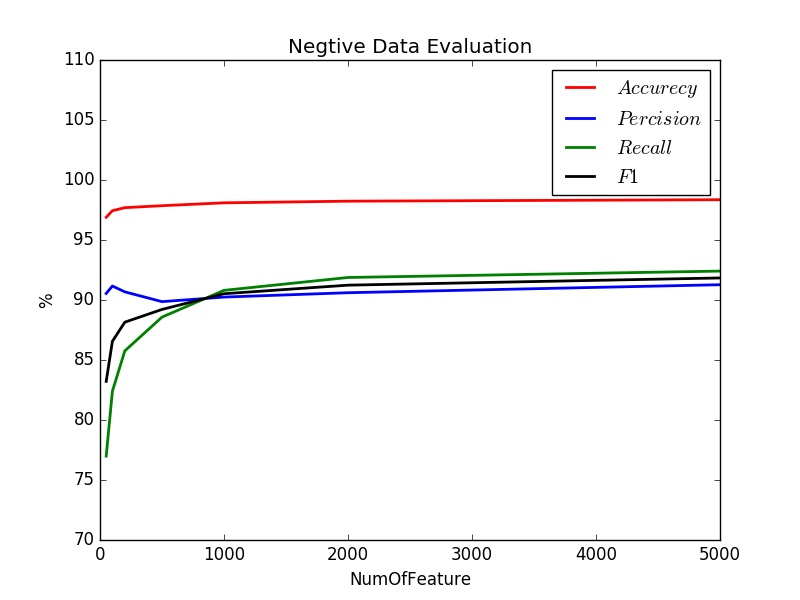
\includegraphics[height=10cm ,width=15cm,angle=0,scale=1]{negtive.jpg}
\caption{\label{Fig:outputfile}Negtive Evaluation } %插入图片的标题,一般放在图片的下方,放在表格的上方
\end{figure}

\begin{figure}
\centering %使插入的图片居中显示
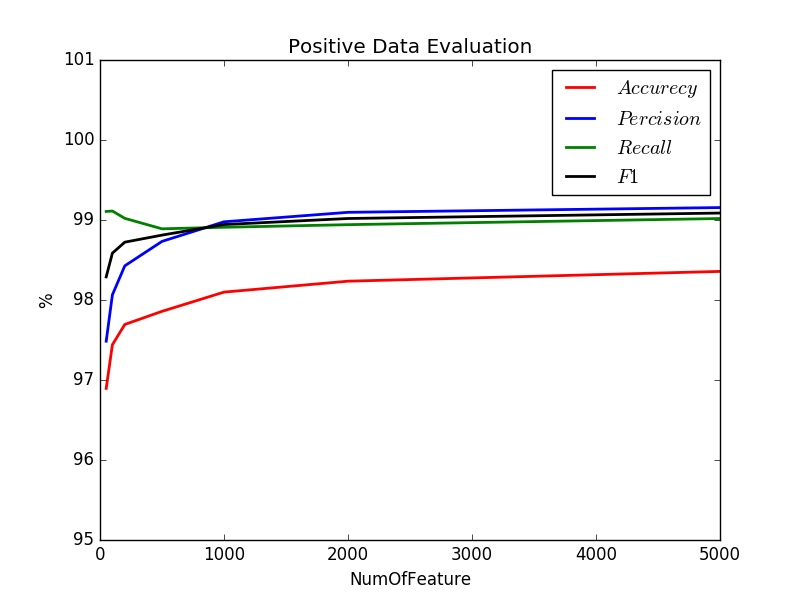
\includegraphics[height=10cm ,width=15cm,angle=0,scale=1]{positive.jpg}
\caption{\label{Fig:outputfile}Positive Evaluation } %插入图片的标题,一般放在图片的下方,放在表格的上方
\end{figure}


\begin{comment}
\begin{table}\label{result}
  \begin{center}
    \begin{tabular}{|c|c|c|c|c|c|c|c|}
    \hline
    \multicolumn{2}{|c|}{} & \multicolumn{2}{|c|}{$F_{Num}$ = 50} &\multicolumn{2}{|c|}{$F_{Num}$ = 105} &\multicolumn{2}{|c|}{$F_{Num}$ = 500} \\ \cline{3-8}
    \multicolumn{2}{|c|}{} & $\lambda = 1.0$ & $\lambda = 10000000$ & $\lambda = 1.0$ & $\lambda = 10000000$ & $\lambda = 1.0$ & $\lambda = 10000000$ \\ \hline
   
         & Percision & 0.9827 & 0.9384& 0.9877 & 0.9404  & 0.9935 &0.9365\\ \cline{2-8}
     1th & Recall & 0.9486 & 0.9557& 0.9477  & 0.9587  & 0.9499 &0.9588\\ \cline{2-8}
         & F1 & 0.9654 &  0.9470& 0.9672 & 0.9495   & 0.9712 &0.9475\\ \hline
         
         & Percision & 0.9836 & 0.9396& 0.9886 & 0.9417   & 0.9939 &0.9373\\ \cline{2-8}
     2th & Recall & 0.9481 & 0.9555& 0.9467 & 0.9586  & 0.9495 &0.9580\\ \cline{2-8}
         & F1 & 0.9655 & 0.9475& 0.9672 & 0.9501   & 0.9712 &0.9475\\ \hline
         
         & Percision & 0.9834 &0.9384& 0.9883 & 0.9402    & 0.9939 &0.9362\\ \cline{2-8}
     3th & Recall & 0.9471 & 0.9547& 0.9472 & 0.9571   & 0.9487 &0.9578\\ \cline{2-8}
         & F1 & 0.9649 & 0.9465& 0.9673 & 0.9486    & 0.9708 &0.9469\\ \hline
         
         & Percision & 0.9829 & 0.9391& 0.9883 & 0.9412   & 0.9940 &0.9369\\ \cline{2-8}
     4th & Recall & 0.9477 & 0.9556 & 0.9472 & 0.9584   & 0.9493 &0.9582\\ \cline{2-8}
         & F1 & 0.9650 & 0.9473& 0.9673 & 0.9497    & 0.9711 &0.9475\\ \hline
         
         & Percision & 0.9836 & 0.9397 & 0.9885 & 0.9416    & 0.9939 &0.9381\\ \cline{2-8}
     5th & Recall & 0.9493 & 0.9564 & 0.9492 & 0.9604    & 0.9497 &0.9587\\ \cline{2-8}
         & F1 & 0.9661 & 0.9480 & 0.9685 & 0.9509   & 0.9713 &0.9483\\ \hline
         
             & Percision & 0.9832 & 0.9391& 0.9882 & 0.9416    & 0.9939 &0.9370\\ \cline{2-8}
     Average & Recall & 0.9482 & 0.9556& 0.9472 & 0.9586    & 0.9494 &0.9583\\ \cline{2-8}
             & F1 & 0.9654 & 0.9472 & 0.9673 & 0.9497   & 0.9711 &0.9475\\ \hline
     
       
    
    \end{tabular}
    \caption{$\lambda$是拉普拉斯平滑参数,$F_{Num}$是取特征词的数量}
  \end{center}
\end{table}
\end{comment}

我们分别对正样例和负样例做5折交叉验证,并计算其Accurecy、Percision、Recall以及F1指标,从图中可以看出Accurecy在选取50个特征值时就已经收敛,而其它三个指标一直等到1000个特征值时才开始收敛。但是由于垃圾短信分类情景来说,Accurecy的可信度并不高,所以我们更加关注于后面三个指标



\end{CJK*}

\end{document}
